\documentclass[12pt]{article}

\tolerance=9999
\emergencystretch=10pt
\hyphenpenalty=10000
\exhyphenpenalty=100
\usepackage[english=nohyphenation]{hyphsubst}

\usepackage{tikz} %% makes the beautiful figures in the document
\usetikzlibrary{shadows}
\usetikzlibrary{shadows.blur}

\usepackage{amsmath} %% Allows inclution of mathematical figures
\usepackage[a4paper,margin=1in]{geometry} %% Responsible for the margin and the headings of the document
\usepackage{mathptmx} %% Times new roman font
\usepackage{booktabs}
\usepackage{tabularx} %% Type of table that allows fragmentation of long sentences inside cells in tables
\usepackage{setspace}
\usepackage{multicol} %% Merging columns in tables
\usepackage{multirow} %% Merging rows in tables
\usepackage{float}
\usepackage{xcolor}
\usepackage{fancyhdr} %% Allows custom heading and footer
\usepackage{lastpage} %% Allows Referencing the last page of the document
\usepackage{calc}
\usepackage{lipsum} %% Random Words
\usepackage{ragged2e}
\usepackage{soul}
\usepackage{tcolorbox}
\usepackage{amssymb}
\usepackage{pgfplots}
\usepackage{tkz-euclide}
\usetikzlibrary{angles}
\usetikzlibrary{intersections,decorations.pathreplacing,positioning}
\usetikzlibrary{arrows.meta}
\usepgfplotslibrary{polar}
\usetikzlibrary{backgrounds}
\usetikzlibrary{positioning}
\pgfplotsset{compat=newest}

\usepackage{amsthm}

\usepgfplotslibrary{fillbetween}
\usetikzlibrary{patterns}

\usepackage{mathtools}

\usepackage{enumitem}


%\usepackage[scaled=1.0]{helvet}             % Load Helvetica
%\renewcommand{\familydefault}{\sfdefault}   % Set Helvetica as main font

\usepackage[T1]{fontenc}


%%%%%%%%%%%%%%%%%%%%%%%%%%%%%%%%%%%%%%%%%%%%%%%%%%%%%%%%%%%%%%%%%%%%%%

\definecolor{h1}{HTML}{196B24}
\definecolor{h2}{HTML}{C1F0C7} %% Allows a custom color in the document using the hex code

%\pagestyle{SILPhdr} %% sets the desired page style of the entire document. Specifically, the headings and footers

\linespread{1.0}

\begin{document}
	\noindent
	{\Large \textbf{9.4.: Arc Length with Parametric Equations}} \\
	\hrule
	
		\begin{enumerate}[label=\arabic*.]
			\item \(x=8t^{\frac{3}{2}}\)\qquad\(y=3+(8-t)^{\frac{3}{2}}\)\qquad\(0\leq t\leq 4\)
		
			\begin{proof}[Solution]
				Get the derivative of the two function in terms of \(t\)
				\begin{align*}
					\frac{dx}{dt} & = \frac{d}{dt}\left(8t^{\frac{3}{2}}\right) = 12t^{\frac{1}{2}} \\
					\frac{dy}{dt} & = \frac{d}{dt}\left(3+\left(8-t\right)^{\frac{3}{2}}\right) = \frac{3}{2}\left(8-t\right)^{\frac{1}{2}}(-1) = -\frac{3}{2}(8-t)^{\frac{1}{2}}
				\end{align*}
				the formula for arc length is
				\begin{align}
					L & = \int_{\alpha}^{\beta} \sqrt{\left(\frac{dx}{dt}\right)^2+\left(\frac{dy}{dt}\right)^2}dt
				\label{eqn:arclengthformula}
				\end{align}
				and,
				\[\alpha = 0\qquad\beta = 4\]
				then,
				\[L = \int_0^4 \sqrt{\left(12t^{\frac{1}{2}}\right)^2+\left(-\frac{3}{2}(8-t)^{\frac{1}{2}}\right)^2}dt\]
				simplifying the integrand,
				\begin{align*}
					L & = \int_0^4 \sqrt{\left(12t^{\frac{1}{2}}\right)^2+\left(-\frac{3}{2}(8-t)^{\frac{1}{2}}\right)^2}~dt \\
					& = \int_0^4 \sqrt{144t+\frac{9}{4}(8-t)}~dt \\
					& = \int_0^4 \sqrt{9\left(16t+\frac{1}{4}(8-t)\right)}~dt \\
					& = \int_0^4 3\sqrt{16t+\frac{1}{4}(8-t)}~dt \\
					& = \int_0^4 3\sqrt{16t+2-\frac{1}{4}t}~dt \\
					& = \int_0^4 3\sqrt{\frac{63}{4}t+2}~dt
				\end{align*}
				let \(u=\frac{63}{4}t+2\), \(du = \frac{63}{4}~dt \Rightarrow \frac{4}{21}~du = 3~dt\)
				\begin{align*}
					L & = \int_0^4 \left(u\right)^{\frac{1}{2}}\left(\frac{4}{21}~du\right) \\
					& = \int_0^4 \frac{4}{21} u^{\frac{1}{2}}~du \\
					& = \left[\frac{4}{21}\left(\frac{2}{3}u^{\frac{3}{2}}\right)\right]_0^4 \\
					& = \left[\frac{8}{63}u^{\frac{3}{2}}\right]_0^4 \\
					& = \left[\frac{8}{63}\left(\frac{63}{4}t+2\right)^{\frac{3}{2}}\right]_0^4 
				\end{align*}
				evaluate,
				\begin{align*}
					L & =  \int_0^4 \sqrt{\left(12t^{\frac{1}{2}}\right)^2+\left(-\frac{3}{2}(8-t)^{\frac{1}{2}}\right)^2}~dt  = \left[\frac{8}{63}\left(\frac{63}{4}t+2\right)^{\frac{3}{2}}\right]_0^4 \\
					& = \left[\frac{8}{63}\left(\frac{63}{4}(4)+2\right)^{\frac{3}{2}}\right]-\left[\frac{8}{63}\left(\frac{63}{4}(0)+2\right)^{\frac{3}{2}}\right] \\
					& = \left[\frac{8}{63}(65)^{\frac{3}{2}}\right]-\left[\frac{8}{63}(2)^{\frac{3}{2}}\right] \\
					& = \frac{8}{63}\left((65)^{\frac{3}{2}}-(2)^{\frac{3}{2}}\right) \\
					& = \frac{8}{63}\left(\sqrt{(65)^3}-\sqrt{(2)^3}\right) \\
					& = \boxed{ \frac{8}{63}\left(\sqrt{274625}-\sqrt{8}\right) \approx 66.18645416}
				\end{align*}
				$\therefore$ The length of the parametric curve is \(66.19\) units in a given range of \(0\leq t\leq 4\)
			\end{proof}
			\hrule
			
			\item[3.] A particle travels along a path defined by the following set of parametric equations. Determine the total distance the particle travels and compare this to the length of the parametric curve itself.
			\[x=4\sin \left(\frac{1}{4}t\right) \qquad y=1-2\cos ^2 \left(\frac{1}{4}t\right) \qquad -52\pi \leq t \leq 34\pi\]
			
			\begin{proof}[Solution]
				Get the derivative of the two function in terms of t
				\begin{align*}
					\frac{dx}{dt} & = \frac{d}{dt}\left(4\sin\left(\frac{1}{4}t\right)\right) = 4\cos\left(\frac{1}{4}t\right)\left(\frac{1}{4}\right) = \cos\left(\frac{1}{4}t\right) \\
					\frac{dy}{dt} & = \frac{d}{dt}\left(1-2\cos^2\left(\frac{1}{4}t\right)\right) \\
					& = (-2)(2)\left(\cos\left(\frac{1}{4}t\right)\right)\left(-\sin \left(\frac{1}{4}t\right)\right)\left(\frac{1}{4}\right) \\
					& = \cos\left(\frac{1}{4}t\right)\sin\left(\frac{1}{4}t\right)
				\end{align*}
				set up the integral
				\[L = \int_{-52\pi}^{34\pi} \sqrt{\left(\cos\left(\frac{1}{4}t\right)\right)^2+\left(\cos\left(\frac{1}{4}t\right)\sin\left(\frac{1}{4}t\right)\right)^2}~dt\]
				simplify the integrand
				\begin{align*}
					L & = \int_{-52\pi}^{34\pi} \sqrt{\cos^2\left(\frac{1}{4}t\right)+\cos^2\left(\frac{1}{4}t\right)\sin^2\left(\frac{1}{4}t\right)}~dt \\
					& = \int_{-52\pi}^{34\pi} \sqrt{\cos^2\left(\frac{1}{4}t\right)\left(1+\sin^2\left(\frac{1}{4}t\right)\right)}~dt \\
					& = \int_{-52\pi}^{34\pi} \cos\left(\frac{1}{4}t\right)\sqrt{1+\sin^2\left(\frac{1}{4}t\right)}~dt
				\end{align*}
				\(-52\pi\leq t \leq 34\pi\) appears to be tracing more than once. Thus, we will change the interval where the curve only traces once. Hence,
				\[-2\pi\leq t \leq 2\pi\]
				then,
				\[L = \int_{-2\pi}^{2\pi} \cos \left(\frac{1}{4}t\right)\sqrt{1+\sin^2\left(\frac{1}{4}t\right)}~dt\]
				substitution method. let
				\[u = \sin \left(\frac{1}{4}t\right)~\Rightarrow~ du = \cos \left(\frac{1}{4}t\right)\left(\frac{1}{4}\right)~dt~\Rightarrow~4~du = \cos \left(\frac{1}{4}t\right)~dt\]
				as for the intervals
				\[t = -2\pi:~u = \sin\left(\frac{1}{4}(-2\pi)\right) = -1 \qquad t=2\pi:~u = \sin\left(\frac{1}{4}(2\pi)\right) = 1\]
				thus the interval is
				\[-1\leq u \leq 1\]
				applying the modifications
				\[L = \int_{-1}^{1} 4\sqrt{1+u^2}~du\]
				let
				\[u = \tan \theta,~ du = \sec^2 \theta~d\theta\] 
				\[u = -1:~ \theta = \tan^{-1}(-1) = -\frac{\pi}{4}\]
				\[u = 1:~ \theta = \tan^{-1}(1) = \frac{\pi}{4}\]
				then,
				\[L = \int_{-\frac{\pi}{4}}^{\frac{\pi}{4}} 4\sqrt{1+\tan^2\theta}\left(\sec^2\theta~d\theta\right)\]
				note that,
				\[1+\tan^2\theta = \sec^2 \theta\]
				then,
				\begin{align*}
					L & = 4\int_{-\frac{\pi}{4}}^{\frac{\pi}{4}} \sqrt{\sec^2\theta}\left(\sec^2\theta~d\theta\right) \\
					& = 4\int_{-\frac{\pi}{4}}^{\frac{\pi}{4}} \sec \theta \sec^2\theta~d\theta \\
					& = 4\int_{-\frac{\pi}{4}}^{\frac{\pi}{4}} \sec^3 \theta~d\theta
				\end{align*}
				to solve the integral, we need the following
				\[\int \sec^n u~du = \frac{1}{n-1} \sec^{n-2}u\tan u +\frac{n-2}{n-1}\int \sec^{n-2}u~du +C\]
				\[\int \sec u~du = \ln|\sec u +\tan u |+C\]
				thus,
				\begin{align*}
					L & = 4 \left[\frac{1}{2} \sec \theta \tan \theta + \frac{1}{2} \int \sec \theta~d\theta\right]_{-\frac{\pi}{4}}^{\frac{\pi}{4}} \\
					& = 4 \left[\frac{1}{2} \sec \theta \tan \theta + \frac{1}{2}\ln |\sec\theta +\tan \theta|\right]_{-\frac{\pi}{4}}^{\frac{\pi}{4}} \\
					& = 4 \cdot \frac{1}{2} \left[\sec \theta \tan \theta +\ln |\sec\theta +\tan \theta|\right]_{-\frac{\pi}{4}}^{\frac{\pi}{4}} \\
					& = 2\left[\sec \theta \tan \theta +\ln |\sec\theta +\tan \theta|\right]_{-\frac{\pi}{4}}^{\frac{\pi}{4}} \\
					& = \boxed{9.18234859757056}
				\end{align*}
				since the curve traces out 21.5 times. Thus the total distance traveled of the particle is
				\[(9.18234859757056)(21.5) = \boxed{197.420494847767}\]
			\end{proof}
			\hrule
			
			\item[5.] Set up, but do not evaluate, an integral that gives the length of the parametric curve given by the following set of parametric equations. You may assume that the curve traces out exactly once for the given range of $t$’s.
			\[x=\cos^3(2t)\qquad y=\sin(1-t^2)\qquad -\frac{3}{2}\leq t \leq 0\]
			
			\begin{proof}[Solution]
				Get the derivative of the two functions in terms of \(t\)
				\begin{align*}
					\frac{dx}{dt} & = \frac{d}{dt}\left(\cos^3(2t)\right) \\
					& = 3\left(\cos^2(2t)\right)\left(-\sin(2t)\right)(2) \\
					& = -6 \cos^2(2t)\sin(2t) \\
					\frac{dy}{dt} & = \frac{d}{dt}\left(\sin(1-t^2)\right) \\
					& = \cos\left(1-t^2\right)(-2t) \\
					& = -2t \cos\left(1-t^2\right)
				\end{align*}
				Using the formula for the Arc length (Eq. \ref{eqn:arclengthformula}) and given that 
				\[\alpha=-\frac{3}{2}\qquad \beta=0\]
				thus,
				\begin{align*}
					L & = \int_{-\frac{3}{2}}^0 \sqrt{\left(-6\cos^2(2t)\sin(2t)\right)^2+\left(-2t\cos\left(1-t^2\right)\right)^2}~dt
				\end{align*}
				simplifying the integrand,
				\begin{align*}
					L & = \int_{-\frac{3}{2}}^0 \sqrt{\left(-6\cos^2(2t)\sin(2t)\right)^2+\left(-2t\cos\left(1-t^2\right)\right)^2}~dt \\
					& = \int_{-\frac{3}{2}}^0 \sqrt{36\cos^4(2t)\sin^2(2t)+4t^2\cos^2\left(1-t^2\right)}~dt \\
					& = \int_{-\frac{3}{2}}^0 \sqrt{4\left(9\cos^4(2t)\sin^2(2t)+t^2\cos^2\left(1-t^2\right)\right)}~dt \\
					& = \int_{-\frac{3}{2}}^0 2\sqrt{9\cos^4(2t)\sin^2(2t)+t^2\cos^2\left(1-t^2\right)}~dt
				\end{align*}
				\begin{center}
					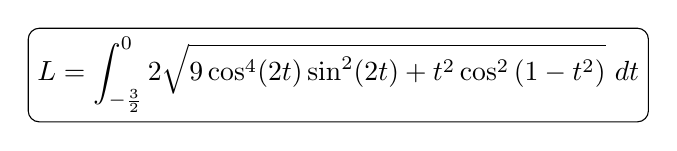
\begin{tikzpicture}
						\node[draw,rectangle,rounded corners]{$\displaystyle L= \int_{-\frac{3}{2}}^0 2\sqrt{9\cos^4(2t)\sin^2(2t)+t^2\cos^2\left(1-t^2\right)}~dt$};
					\end{tikzpicture}
				\end{center}
			\end{proof}
			\hrule
			
	
		\end{enumerate}
	
	\newpage
		\noindent
		{\Large \textbf{9.6.: Polar Coordinates}} \\
		\hrule
		
		\begin{enumerate}
			\item[1.] For the point with polar coordinates \(\left(2,~\frac{\pi}{7}\right)\) determine three different sets of coordinates for the same point all of which have angles different from \(\frac{\pi}{7}\) and are in the range \(-2\pi\leq \theta \leq 2\pi\)
			
			\begin{proof}[Solution]
				Graph
				\begin{center}
					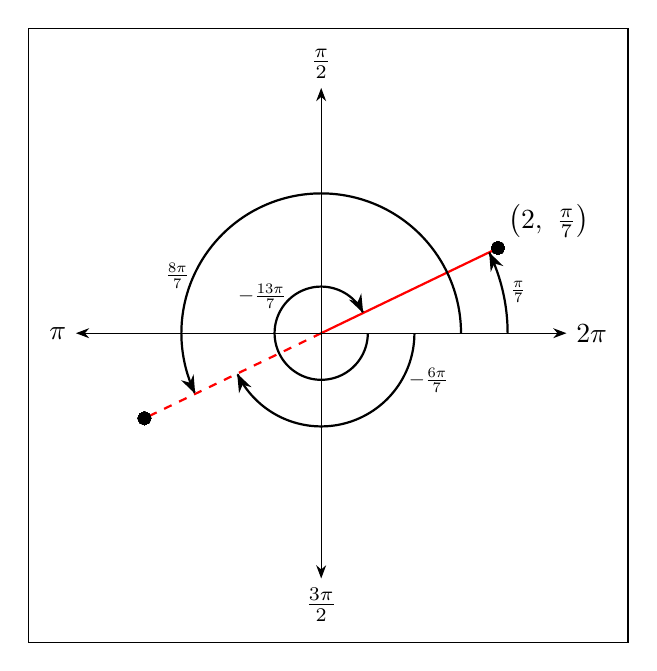
\begin{tikzpicture}[show background rectangle]
						\begin{polaraxis}[clip=false,xticklabels={ , , , , , , , },axis x line=none,axis y line=none,yticklabels={ , , , , , , , }]
							\addplot[domain=0:2,samples=100,thick,red] ({180/7},{x});
							\addplot[domain=0:2,samples=100,thick,red,dashed] ({(180/7)+180},{x});
							\addplot[domain=-2.5:2.5,samples=100,black,Stealth-Stealth] ({0},{x}) node[anchor=west,pos=1]{\(2\pi\)} node[anchor=east,pos=0]{\(\pi\)};
							\addplot[domain=-2.5:2.5,samples=100,black,Stealth-Stealth] ({90},{x}) node[anchor=south,pos=1]{\(\frac{\pi}{2}\)} node[anchor=north,pos=0]{\(\frac{3\pi}{2}\)};
							\addplot[domain=0:(180/7),samples=300,thick,-Stealth] {1.9} node[anchor=west,pos=0.5,scale=0.75]{\(\frac{\pi}{7}\)};
							\addplot[domain=0:-13*(180/7),samples=300,thick,-Stealth] {0.475} node[anchor=south east,pos=0.7,scale=0.75,yshift=-10px]{\(-\frac{13\pi}{7}\)};
							\addplot[domain=0:-6*(180/7),samples=300,thick,-Stealth] {0.95} node[anchor=north west,pos=0.2,scale=0.75,yshift=10px]{\(-\frac{6\pi}{7}\)};
							\addplot[domain=0:8*(180/7),samples=300,thick,-Stealth] {1.425} node[anchor=south east,pos=0.8,scale=0.75,xshift=5px]{\(\frac{8\pi}{7}\)};
							\addplot[domain=0:2,thick,black,mark=*] ({(180/7)},{2}) node[anchor=south west,pos=1]{\(\left(2,~\frac{\pi}{7}\right)\)};;
							\addplot[domain=0:2,thick,black,mark=*] ({(180/7)+180},{2}) ;
						\end{polaraxis}
					\end{tikzpicture}
				\end{center}
				we get the reflection point of the point through its angle,
				\[\frac{\pi}{7}+\pi=\frac{8\pi}{7}\]
				Now, we have the two positive angles which are
				\[\frac{\pi}{7},\qquad \frac{8\pi}{7}\]
				For the negatives,
				\[-2\pi+\frac{\pi}{7}=-\frac{13\pi}{7},\qquad -2\pi+\frac{8\pi}{7}=-\frac{6\pi}{7}\]
				Constructing the polar coordinates for the given point, we found that,
				\[\left(2,~\frac{\pi}{7}\right) = \left(2,~-\frac{13\pi}{7}\right)\]
				If we are going to use \(r=-2\), then its polar coordinates are,
				\begin{center}
					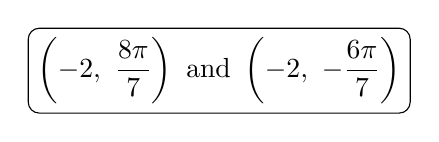
\begin{tikzpicture}
						\node[draw,rectangle,rounded corners]{$\displaystyle \left(-2,~\frac{8\pi}{7}\right)~\text{and}~\left(-2,~-\frac{6\pi}{7}\right)$};
					\end{tikzpicture}
				\end{center}
				you can still use this alternative polar coordinates since it refers to the same given point, the difference is, if \(r=-2\), the angle now measures from \(\pi\)
				\begin{center}
					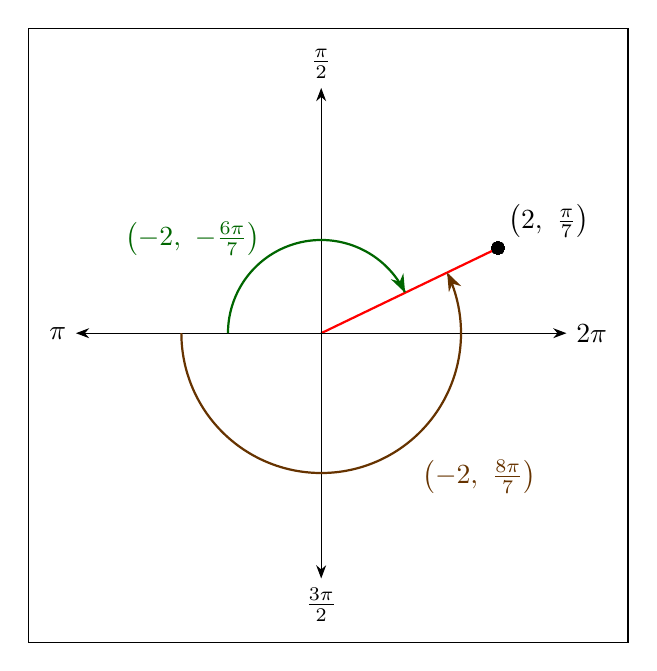
\begin{tikzpicture}[show background rectangle]
						\begin{polaraxis}[clip=false,xticklabels={ , , , , , , , },axis x line=none,axis y line=none,yticklabels={ , , , , , , , }]
							\addplot[domain=0:2,samples=100,thick,red] ({180/7},{x});
							\addplot[domain=-2.5:2.5,samples=100,black,Stealth-Stealth] ({0},{x}) node[anchor=west,pos=1]{\(2\pi\)} node[anchor=east,pos=0]{\(\pi\)};
							\addplot[domain=-2.5:2.5,samples=100,black,Stealth-Stealth] ({90},{x}) node[anchor=south,pos=1]{\(\frac{\pi}{2}\)} node[anchor=north,pos=0]{\(\frac{3\pi}{2}\)};
							\addplot[domain=0:2,thick,black,mark=*] ({(180/7)},{2}) node[anchor=south west,pos=1]{\(\left(2,~\frac{\pi}{7}\right)\)};
							\addplot[domain=180:8*(180/7)+180,samples=300,thick,-Stealth,orange!40!black] {1.425} node[anchor=north west,pos=0.6,xshift=5px]{\(\left(-2,~\frac{8\pi}{7}\right)\)};
							\addplot[domain=-180:-6*(180/7)-180,samples=300,thick,-Stealth,green!40!black] {0.95} node[anchor=south east,pos=0.3,xshift=5px]{\(\left(-2,~-\frac{6\pi}{7}\right)\)};
						\end{polaraxis}
					\end{tikzpicture}
				\end{center}
			\end{proof}
			\hrule
			
			\item[3.] The Cartesian coordinate of a point are \((2,~-6)\). Determine a set of polar coordinates for the point.
			
			\begin{proof}[Solution]
				Determine \(r\) which is expressed by
				\[r^2 = x^2+y^2\qquad \Longrightarrow \qquad r=\sqrt{x^2+y^2}\]
				since,
				\[x=2,\qquad y=-6\]
				then,
				\[r= \sqrt{(2)^2+(-6)^2}=\sqrt{40}=\sqrt{4\cdot10}=2\sqrt{10}\]
				For the angles, we have two ways. Thus, we have two angles as well. The angle is defined as
				\[\theta_1=\tan^{-1}\left(\frac{y}{x}\right)\quad \text{OR} \quad \theta_2=\theta_1+\pi\]
				then,
				\begin{align*}
					\theta_1 & = \tan^{-1}\left(\frac{y}{x}\right) \\
					& = \tan^{-1}\left(\frac{-6}{2}\right) = -1.249 \\
					\theta_2 & = \theta_1 +\pi \\
					& = -1.249 + \pi \approx 1.893
				\end{align*}
				referring to the given coordinate, that is \((2,-6)\), the point falls on quadrant 4. Therefore, we must choose an angle that also falls on the 4th quadrant. Analyzing both angles, \(\theta_1\) falls on quadrant 4. Thus, our polar coordinates is
				\begin{center}
					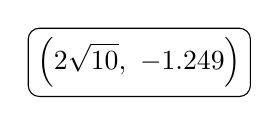
\begin{tikzpicture}
						\node[draw,rectangle,rounded corners]{$\displaystyle \left(2\sqrt{10},~-1.249\right)$};
					\end{tikzpicture}
				\end{center}
			\end{proof}
			\hrule
			
			\item[5.] Convert the given equation into an equation in terms of polar coordinates.
				\[\frac{4x}{3x^2+3y^2} = 6-xy\]
				
				\begin{proof}[Solution]
					Note the following expressions
					\[x=r\cos \theta\qquad y=r\sin \theta\qquad r^2=x^2+y^2\]
					Looking at the equation, we have
					\[3x^2+3y^2~ \Longrightarrow ~ 3\left(x^2+y^2\right) ~ \Longrightarrow ~ 3r^2\]
					and the rest of the variables in the equation, we will substitute it with the aforementioned expressions. Then,
					\begin{align*}
						\frac{4x}{3r^2} & = 6-xy \\
						\frac{4\left(r\cos \theta\right)}{3r^2} & = 6-\left(r\cos \theta\right)\left(r\sin \theta\right)
					\end{align*}
					\begin{center}
						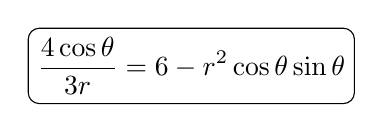
\begin{tikzpicture}
							\node[draw,rectangle,rounded corners]{$\displaystyle \frac{4\cos \theta}{3r} = 6-r^2\cos \theta \sin \theta$};
						\end{tikzpicture}
					\end{center}
				\end{proof}
				\hrule
			
			\item[7.] Convert the given equation into an equation in terms of Cartesian coordinates.
				\[6r^3 \sin \left(\theta\right) = 4- \cos \theta\]
				
				\begin{proof}[Solution]
					Note the following expressions
					\[x=r\cos \theta\qquad y=r\sin \theta\qquad r=\sqrt{x^2+y^2}\]
					since the equation does not have any similar formats as in the above expressions. We multiply it by \(r\). Thus,
					\[6r^4\sin\left(\theta\right) = 4r-r\cos \theta ~\Longrightarrow~ 6r^3 \left(r\sin\left(\theta\right)\right)=4r-r\cos\theta\]
					then, 
					\begin{center}
						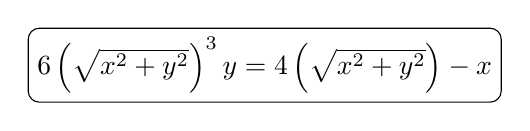
\begin{tikzpicture}
						\node[draw,rectangle,rounded corners]{$6\left(\sqrt{x^2+y^2}\right)^3y = 4\left(\sqrt{x^2+y^2}\right)-x$};
					\end{tikzpicture}
					\end{center}
				\end{proof}
				\hrule
			
			\item[9.] Sketch the graph of the given polar equation.
				\[\cos \left(\theta\right) = \frac{6}{r}\]
				
				\begin{proof}[Solution]
					Given the equation
					\[\cos\left(\theta\right)=\frac{6}{r}\]
					we can rewrite it as
					\[r\cos\left(\theta\right)=6\]
					since, \(r\cos\left(\theta\right)=x\). Thus,
					\[x=6\]
					\begin{center}
						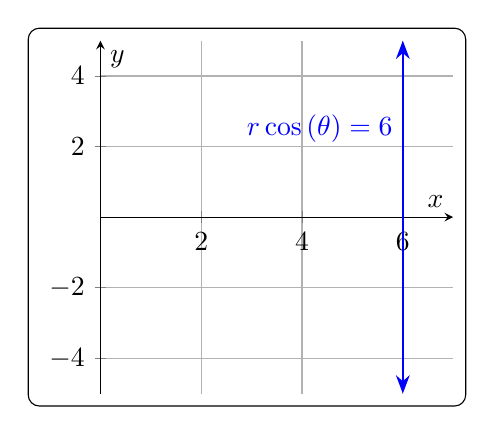
\begin{tikzpicture}[show background rectangle,rounded corners]
						\begin{axis}[axis x line=center,
							axis y line=center,
							xmajorgrids,
							x grid style={black!30},
							ymajorgrids,
							y grid style={black!30},
							xlabel=$x$,
							ylabel=$y$,
							width=0.5\linewidth,
							height=0.5\linewidth,
							ymax=5,ymin=-5,
							xmax=7,xmin=0
							]
							
							\addplot+[mark=none,blue,thick,Stealth-Stealth] coordinates {(6,-5)(6,5)} node[anchor=east,pos=0.75]{\(r\cos \left(\theta\right)=6\)};
						\end{axis}
					\end{tikzpicture}
					\end{center}
				\end{proof}
			
		\end{enumerate}
	\newpage
		\noindent
		{\Large \textbf{9.7.: Tangents with Polar Coordinates}} \\
		\hrule
		
		\begin{enumerate}
			\item[1.] Find the tangent line to \(r=\sin \left(4\theta\right)\sin\left(\theta\right)\) at \(\theta=\frac{\pi}{6}\).
			
			\begin{proof}[Solution]
				Get the derivative of \(r\) in terms of \(\theta\)
				\begin{align*}
					\frac{dr}{d\theta} & = \frac{d}{d\theta} \left(\sin\left(4\theta\right)\cos \left(\theta\right)\right) \\
					& = \cos\left(4\theta\right)(4)\cos \left(\theta\right)+\left(-\sin\left(\theta\right)\right)\left(\sin\left(4\theta\right)\right) \\
					& = 4\cos\left(4\theta\right)\cos\left(\theta\right)-\sin\left(\theta\right)\sin\left(4\theta\right)
				\end{align*}
				The formula for the derivative with polar coordinates is expressed by
				\[\frac{dy}{dx} = \frac{\frac{dr}{d\theta}\sin\left(\theta\right)+r\cos\left(\theta\right)}{\frac{dr}{d\theta}\cos\left(\theta\right)-r\sin\left(\theta\right)}\]
				then,
				\begin{align*}
					\frac{dy}{dx} & = \frac{\left(4\cos\left(4\theta\right)\cos\left(\theta\right)-\sin\left(\theta\right)\sin\left(4\theta\right)\right)\sin\left(\theta\right)+\left(\sin\left(4\theta\right)\cos\left(\theta\right)\right)\cos\left(\theta\right)}{\left(4\cos\left(4\theta\right)\cos\left(\theta\right)-\sin\left(\theta\right)\sin\left(4\theta\right)\right)\cos\left(\theta\right)-\left(\sin\left(4\theta\right)\cos\left(\theta\right)\right)\sin\left(\theta\right)} \\
					& = \frac{4\cos\left(4\theta\right)\cos\left(\theta\right)\sin\left(\theta\right)-\sin^2\left(\theta\right)\sin\left(4\theta\right)+\sin\left(4\theta\right)\cos^2\left(\theta\right)}{4\cos\left(4\theta\right)\cos^2\left(\theta\right)-\sin\left(\theta\right)\sin\left(4\theta\right)\cos\left(\theta\right)-\sin\left(4\theta\right)\sin\left(\theta\right)\cos\left(\theta\right)}
				\end{align*}
				Now, we get the slope of the tangent line
				\begin{align*}
					m & = \left[\frac{dy}{dx}\right]_{\theta=\frac{\pi}{6}} \\
					& = \left[\frac{4\cos\left(4\theta\right)\cos\left(\theta\right)\sin\left(\theta\right)-\sin^2\left(\theta\right)\sin\left(4\theta\right)+\sin\left(4\theta\right)\cos^2\left(\theta\right)}{4\cos\left(4\theta\right)\cos^2\left(\theta\right)-\sin\left(\theta\right)\sin\left(4\theta\right)\cos\left(\theta\right)-\sin\left(4\theta\right)\sin\left(\theta\right)\cos\left(\theta\right)}\right]_{\theta=\frac{\pi}{6}} \\
					& = \frac{4\cos\left(4\left(\frac{\pi}{6}\right)\right)\cos\left(\frac{\pi}{6}\right)\sin\left(\frac{\pi}{6}\right)-\sin^2\left(\frac{\pi}{6}\right)\sin\left(4\left(\frac{\pi}{6}\right)\right)+\sin\left(4\left(\frac{\pi}{6}\right)\right)\cos^2\left(\frac{\pi}{6}\right)}{4\cos\left(4\left(\frac{\pi}{6}\right)\right)\cos^2\left(\frac{\pi}{6}\right)-\sin\left(\frac{\pi}{6}\right)\sin\left(4\left(\frac{\pi}{6}\right)\right)\cos\left(\frac{\pi}{6}\right)-\sin\left(4\left(\frac{\pi}{6}\right)\right)\sin\left(\frac{\pi}{6}\right)\cos\left(\frac{\pi}{6}\right)} \\
					& = \frac{\sqrt{3}}{9}
				\end{align*}
				Evaluate \(r\) by \(\theta=\frac{\pi}{6}\)
				\begin{align*}
					r & = \left[\sin\left(4\theta\right)\cos\left(\theta\right)\right]_{\theta=\frac{\pi}{6}} \\
					& = \sin\left(4\left(\frac{\pi}{6}\right)\right)\cos\left(\frac{\pi}{6}\right) \\
					& = \frac{3}{4}
				\end{align*}
				Get the coordinates for \(r\)
				\begin{align*}
					x & = r\cos\left(\theta\right) = \frac{3}{4}\cos\left(\frac{\pi}{6}\right) = \frac{3\sqrt{3}}{8} \\
					y & = r\sin\left(\theta\right) = \frac{3}{4}\sin\left(\frac{\pi}{6}\right) = \frac{3}{8}
				\end{align*}
				we construct the function for the tangent line
				\begin{align*}
					y-y_1 & =m\left(x-x_1\right) \\
					y & =m\left(x-x_1\right)+y_1
				\end{align*}
				\begin{center}
					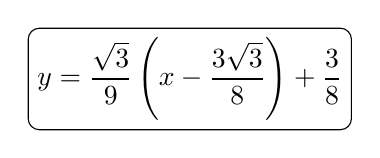
\begin{tikzpicture}
						\node[draw,rectangle,rounded corners]{$\displaystyle y=\frac{\sqrt{3}}{9}\left(x-\frac{3\sqrt{3}}{8}\right)+\frac{3}{8}$};
					\end{tikzpicture}
				\end{center}
			\end{proof}
			
		\end{enumerate}
	
	\newpage
	\noindent
	{\Large \textbf{9.9.: Arc Lengths with Polar Coordinates}} \\
	\hrule
	
		\begin{enumerate}
			\item[1.] \(\displaystyle r = -4\sin \left(\theta\right),~0\leq \theta \leq \pi\)
			
			\begin{proof}[Solution]
				\begin{align*}
					\frac{dr}{d\theta} & = \frac{d}{d\theta} \left(-4\sin\left(\theta\right)\right) = -4\cos\left(\theta\right) \\
					ds & = \sqrt{\left(-4\sin\left(\theta\right)\right)^2+\left(-4\cos\left(\theta\right)\right)^2}~d\theta \\
					& = \sqrt{16\sin^2\left(\theta\right)+16\cos^2\left(\theta\right)}~d\theta \\
					& = \sqrt{16\left(\sin^2\left(\theta\right)+\cos^2\left(\theta\right)\right)}~d\theta \\
					& = 4\sqrt{(1)}~d\theta && \text{n.b.:}~\sin^2\theta+\cos^2\theta = 1 \\
					ds & = 4~d\theta \\
					L & = \int_)^{\pi} 4~d\theta = \left[4\theta\right]_0^{\pi} = \left[4\pi\right]-\left[4(0)\right] = 4\pi
				\end{align*}
				\begin{center}
					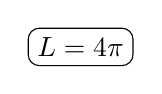
\begin{tikzpicture}
						\node[draw,rectangle,rounded corners]{$\displaystyle L = 4\pi$};
					\end{tikzpicture}
				\end{center}
			\end{proof}
			\hrule
			
			\item[3.] \(\displaystyle r=\cos\left(2\theta\right)+\sin\left(3\theta\right),~0\leq \theta\leq 2\pi\)
			\begin{proof}[Solution]
				\begin{align*}
					\frac{dr}{d\theta} & = \frac{d}{d\theta} \left(\cos\left(2\theta\right)+\sin\left(3\theta\right)\right) \\
					& = -\sin\left(2\theta\right)\left(2\right)+\cos \left(3\theta\right)\left(3\right) \\
					& = -2\sin\left(2\theta\right)+3\cos\left(3\theta\right) \\
					ds & = \sqrt{r^2+\left(\frac{dr}{d\theta}\right)^2}~d\theta \\
					& = \sqrt{\left(\cos\left(2\theta\right)+\sin\left(3\theta\right)\right)^2+\left(-2\sin\left(2\theta\right)+3\cos\left(3\theta\right)\right)^2}~d\theta \\
					L & = \int_0^{2\pi} \sqrt{\left(\cos\left(2\theta\right)+\sin\left(2\theta\right)\right)^2+\left(-2\sin\left(2\theta\right)+3\cos\left(3\theta\right)\right)^2}~d\theta
				\end{align*}
				\begin{center}
					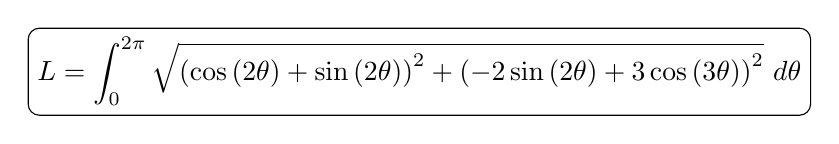
\begin{tikzpicture}
						\node[draw,rectangle,rounded corners]{$\displaystyle L = \int_0^{2\pi} \sqrt{\left(\cos\left(2\theta\right)+\sin\left(2\theta\right)\right)^2+\left(-2\sin\left(2\theta\right)+3\cos\left(3\theta\right)\right)^2}~d\theta$};
					\end{tikzpicture}
				\end{center}
			\end{proof}
		\end{enumerate}
	
\end{document}